\documentclass[../main.tex]{subfiles}
 
\begin{document}

\subsection{Introduction to Finite Element Method}

Finite difference method has two main limitations cause by the "rectangle" it utilizes. The size of rectangles are similar so there is no way to handle curved/irregularly shaped domain ,or emphasize some area for more detail.

So there comes \textbf{Finite Element Method (FEM)}, it subdivides a large problem domain into smaller and simpler pieces (polygons) that are called finite elements. The simple equations that model these finite elements are then assembled into a larger system of equations that models the entire problem. FEM then uses variational methods from the calculus of variations to approximate a solution by minimizing an associated error function.

FEM is best understood from its practical application, known as \textbf{Finite Element Analysis (FEA)}. FEA as applied in engineering is a computational tool for performing engineering analysis. It includes the use of mesh generation techniques for dividing a complex problem into small elements, as well as the use of software program coded with FEM algorithm. In applying FEA, the complex problem is usually a physical system with the underlying physics such as the Euler-Bernoulli beam equation, the heat equation, or the Navier-Stokes equations expressed in either PDE or integral equations, while the divided small elements of the complex problem represent different areas in the physical system.

FEA is a good choice for analyzing problems over complicated domains (like cars and oil pipelines), when the domain changes (as during a solid state reaction with a moving boundary), when the desired precision varies over the entire domain, or when the solution lacks smoothness. FEA simulations provide a valuable resource as they remove multiple instances of creation and testing of hard prototypes for various high fidelity situations. For instance, in a frontal crash simulation it is possible to increase prediction accuracy in "important" areas like the front of the car and reduce it in its rear (thus reducing cost of the simulation).

Let's consider the Dirichlet problem for Poisson's equation in the plane:
\begin{equation} \label{eq:FEM1}
    \begin{split}
     - \, \Delta u & = f \text{ in } D \\
    u & = 0 \text{ on bdy } D
    \end{split}
\end{equation}

$D$ is triangulated by be approximated by a region $D_N$, which is the union of a finite number of triangles (see fig.\ref{fig:FEM1}). Let the interior vertices be donated by $V_1,...,V_N$.

\begin{figure}[h]
    \caption{Illustration of triangles when $N = 1$ and $N = 7$)}
    \centering
    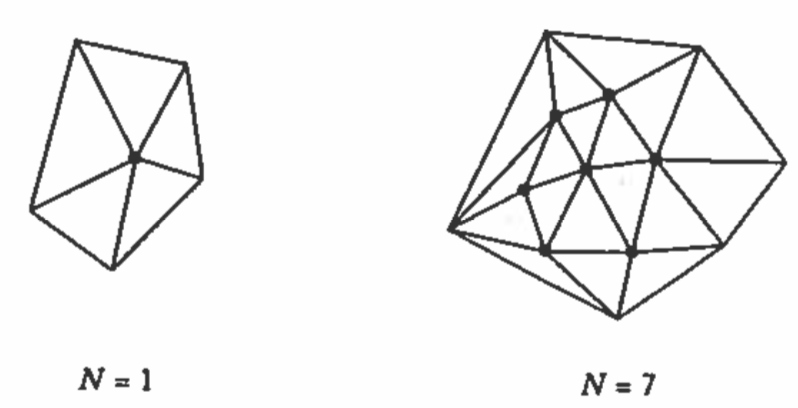
\includegraphics[width=6cm]{images/FEM1.png}
    \label{fig:FEM1}
\end{figure}

Next, we pick $N$ trial functions, $v_1(x,y),...,v_N(x,y)$, one for each interior vertex. Each trial function $v_i(x,y)$ is chosen to equal 1 at its vertex $V_i$ and to equal 0 at all the other vertices (see fig.\ref{fig:FEM2}). Inside each triangle, each trial function is a linear function: $v_i(x,y) = a + b \, x + c \, y$. (The coefficients $a$, $b$, $c$ are different for each trial function and for each triangle.) This prescription determines $v_i(x,y)$ uniquely. In fact, its graph is simply a pyramid of unit height with its summit at $V_i$ and it is identically zero on all the triangles that do not touch $V_i$.

\begin{figure}[h]
    \caption{Illustration of triangles when $N = 1$ and $N = 7$)}
    \centering
    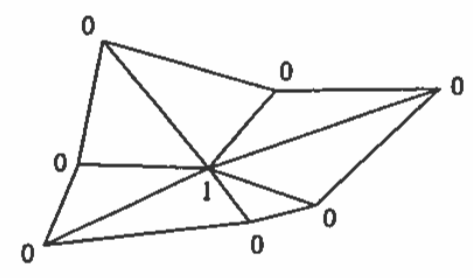
\includegraphics[width=6cm]{images/FEM2.png}
    \label{fig:FEM2}
\end{figure}

We shall approximate the solution $u(x,y)$ by a linear combination of the $v_i(x,y)$:
\begin{equation}
    u_N(x,y) = U_1 \, v_1(x,y) + ... + U_N \, v_N(x,y) \label{eq:FEM2}
\end{equation}

To motivate our choice we need a degression. Let's rewrite problem in eq.\ref{eq:FEM1} using Green's first identity [formula (GI) from Section 7.1]. We multiply Poisson's equation by any function $v(x,y)$ that vanishes on the boundary. Then:
\begin{equation}
    \iint_D \nabla u \, \nabla v \, \mathrm{d}x \, \mathrm{d}y = \iint_D f \, v \, \mathrm{d}x \, \mathrm{d}y \label{eq:FEM3}
\end{equation}

Rather than requiring eq.\ref{eq:FEM3} to be valid for $u_N(x,y)$ for all functions $v(x,y)$, we ask only that it be valid for the first $N$ special trial functions $v = v_j \, (j = 1,...,N)$. Thus, with $u(x,y) = u_N(x,y)$ and $v(x,y) = v_j(x,y)$, eq.\ref{eq:FEM3} becomes:
\begin{equation}
    \sum_{i=1}^N \, U_i \, \left( \iint_D \nabla v_i \, \nabla v_j \, \mathrm{d}x \, \mathrm{d}y \right) = \iint_D f \, v_j \, \mathrm{d}x \, \mathrm{d}y \label{eq:FEM4}
\end{equation}

This is a system of $N$ linear equation $(j = 1,...,N)$ in the $N$ unknowns $U_1,...,U_N$. If we denote:
\begin{equation}
    m_{ij} = \iint_D \nabla v_i \, \nabla v_j \, \mathrm{d}x \, \mathrm{d}y \quad \text{and} \quad f_j = \iint_D f \, v_j \, \mathrm{d}x \, \mathrm{d}y \label{eq:FEM4}
\end{equation}
then the system takes the form:
\begin{equation}
    \sum_{i=1}^N \, m_{ij} \, U_i = f_i \quad (j = 1,...,N) \label{eq:FEM5}
\end{equation}

The finite element method consists of calculating $m_{ij}$ and $f_j$ from eq.\ref{eq:FEM4} and solving eq.\ref{eq:FEM5}. The approximate solution $u_N$ automatically vanishes on the boundary of $D_N$. Notice also that, at a vertex $V_k = (x_k,y_k)$,
\begin{equation}
    u_N(x_k,y_k) = U_1 \, v_1(x_k,y_k) + ... + U_N \, v_N(x_k,y_k) = U_k
\end{equation}
since $v_i(x_k,y_k)$ equals 0 for $i \neq k$. Thus the coefficients are precisely the values of the qpproximate solution at the vertices.

\end{document}